\documentclass[fleqn, 10pt]{article}

\usepackage[utf8]{inputenc}
\usepackage[spanish]{babel}
\usepackage{amsthm}
\usepackage{nccmath}
\usepackage{enumitem}
\usepackage{graphicx}
\usepackage{verbatim}
\usepackage{algpseudocode}



\theoremstyle{plain}
\newtheorem{proposicion}{Proposición}

\theoremstyle{definition}
\newtheorem{definition}{Definición}[section]
\newtheorem{example}{Ejemplo}[section]


\title{Teoría de Autómatas y Lenguajes Formales\\[.4\baselineskip]Práctica 3.}
\author{Carlos Velasco Hilario}
\date{13/12/2022}


\begin{document}

\maketitle

\section{Define the TM solution of exercise 3.4 of the problem list and test its correct behaviour. }

\begin{center}
\includegraphics[width=11cm, height=8cm]{ejercicio1practica2.png}
\end{center}
\section {Define a recursive function for the sum of three values.}

\begin{equation}
suma <<\pi^1_1|\sigma(\pi^3_3)>|\sigma(\pi^4_4)>
\end {equation}

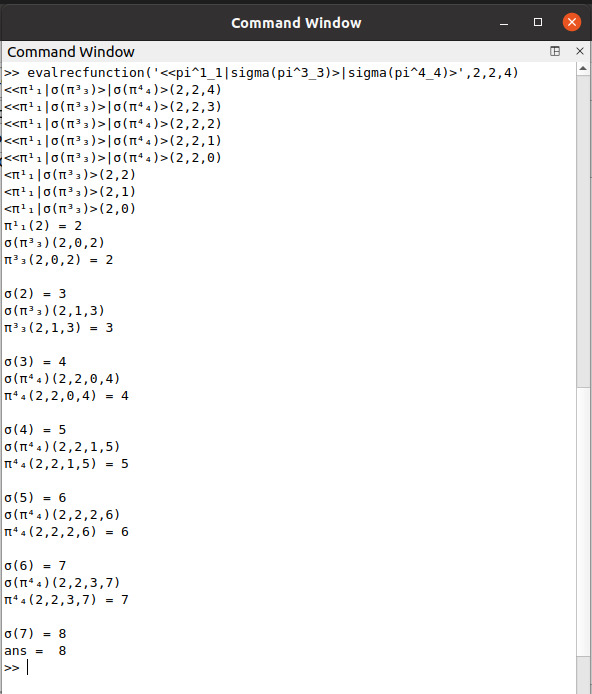
\includegraphics[width=11cm, height=8cm] {practica3ej2.png}

\begin{center}
\end{center}
\section {Implement a WHILE program that computes the sum of three values. You must use an auxiliary variable that accumulates the result of the sum.}
\begin{algorithmic}
\While{X1!=0 }
\While{X2!=0 }

	\\x3:=x3+1;
	\\x2:=x2-1;
\EndWhile
\\x3:=x3+1;
\\x1:=x1-1;
\EndWhile
\end{algorithmic}
\end{document}